% 1977 年宁夏卷第 13 题：圆内接三角形 ABC，AB、BC 边上的高 CE、AD 相交于 H，
% AD 延长线交弧 BC 于 F，连线 FC 为虚线；角 1 在 B、角 2 在 C、角 3 在 H、角 4 在 F（按源卷第 3 页布局）
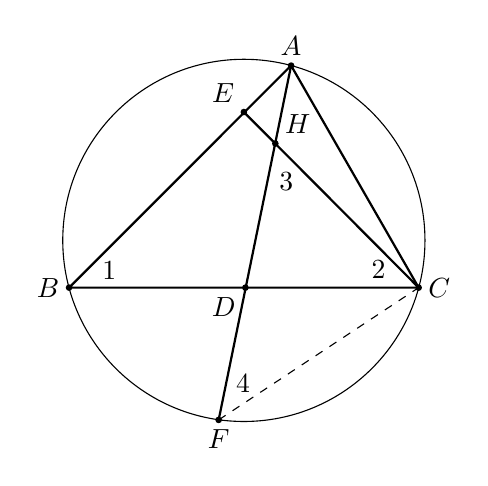
\begin{tikzpicture}[scale=1.0]
  \draw (2.6,2.1) circle (2.3);
  \coordinate (A) at (3.2,4.32);
  \coordinate (B) at (0.38,1.5);
  \coordinate (C) at (4.82,1.5);
  \coordinate (D) at (2.62,1.5);
  \coordinate (E) at (2.6,3.73);
  \coordinate (H) at (3.0,3.33);
  \coordinate (F) at (2.28,-0.18);
  \draw[thick] (A)--(B)--(C)--cycle;
  \draw[thick] (A)--(F);
  \draw[thick] (C)--(E);
  \draw[dashed] (F)--(C);
  \fill (A) circle (1.2pt) node[above] {$A$};
  \fill (B) circle (1.2pt) node[left] {$B$};
  \fill (C) circle (1.2pt) node[right] {$C$};
  \fill (D) circle (1.2pt) node[below left] {$D$};
  \fill (E) circle (1.2pt) node[above left] {$E$};
  \fill (H) circle (1.2pt) node[above right] {$H$};
  \fill (F) circle (1.2pt) node[below] {$F$};
  \node at (0.89,1.72) {$1$};
  \node at (4.31,1.73) {$2$};
  \node at (3.14,2.85) {$3$};
  \node at (2.59,0.28) {$4$};
\end{tikzpicture}
